\documentclass[../besoin_sys.tex]{subfiles}
\begin{document}
\section{Lobby}

Au lancement d'une partie, l'interface du lobby est affiché. On peut à ce moment inviter de nouveaux joueurs. 
Le lobby est joignable par d'autres joueurs sans nécessairement avoir envoyé d'invitations.
Comme dit précédemment, le joueur principal est le premier joueur à avoir rejoint le lobby, le second joueur est le second joueur à avoir rejoint le lobby, et les autres joueurs sont des spectateurs.


\begin{figure}[h]
    \centering
    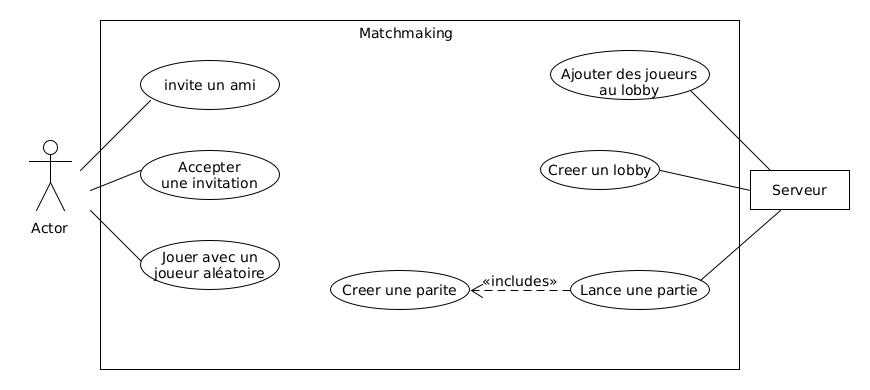
\includegraphics[scale=0.6]{img_fonctionnel/usecas_sys_matchmaking.png}
    \label{fig:Lobby}
    \caption{Lobby}
\end{figure}
\end{document}